\subsection*{Classes}

In order to construct a software model for the performance functional, a few things need to be taken into account. 
First, a performance functional can be measured on a data set, on a mathematical model or on both of them. 
Second, a performance functional might be composed by three terms: an objective functional, a regularization functional and a constraints functional. 
Third, sometimes we will need numerical differentiation to calculate the derivatives of the performance with respect to the parameters in the neural network.

\begin{description}

\item[Data set] The class which represents the concept of data set is called \lstinline"DataSet". This class is basically a data matrix with information on the variables (input or target) and the instances (training, generalization or testing).

\item[Mathematical model] The class representing the concept of mathematical model is called \lstinline"MathematicalModel". 
This is a very abstract class for calculating the solution of some mathematical model for a given input to that model. 

\item[Performance term] The class which represents the concepts of objective, regularization and constraints terms is called \lstinline"PerformanceTerm". 
The objective functional is the most important term in the performance functional expression. 

\item[Numerical differentiation] The class with utilities for numerical differentiation is called \lstinline"NumericalDifferentiation".
While it is not needed for data modelling problems, it is in general a must when solving optimal control, optimal shape design or inverse problems. 

\item[Performance functional] The class which represents the concept of performance functional is called \lstinline"PerformanceFunctional". 
A performance functional is defined as the sum of the objective, regularization and constraints functionals. 

\end{description}


\subsection*{Associations}

The associations among the concepts described above are the following:

\begin{description}
\item[Performance functional - Data set] A performance functional might be measured on a data set.  

\item[Performance functional - Mathematical model] A performance functional might be measured on a mathematical model. 

\item[Performance functional - Objective functional] A performance functional might contain an objective term. 

\item[Performance functional - Regularization functional] A performance functional might contain a regularization term.

\item[Performance functional - Constraints functional] A performance functional might contain a constraints term.
\end{description}

Figure \ref{PerformanceFunctionalAssociationDiagram} depicts an association diagram for the performance functional class. 

\begin{figure}[h!]
\begin{center}
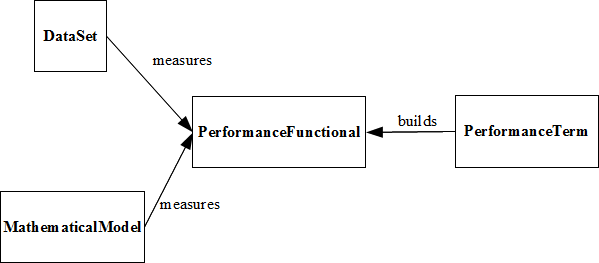
\includegraphics[width=1.0\textwidth]{performance_functional/performance_functional_association_diagram}
\caption{Association diagram for the \lstinline'PerformanceFunctional' class.}\label{PerformanceFunctionalAssociationDiagram}
\end{center}
\end{figure}

\subsection*{Derived classes}

The next task is then to establish which classes are abstract and
to derive the necessary concrete classes to be added to the
system. Let us then examine the classes we have so far:

\begin{description}

\item[Data set] This is called \lstinline"DataSet", and it is a concrete class. 
It can be instantiated by loading the data matrix from a file and setting the variables and instances information. 

\item[Mathematical model] The class \lstinline"MathematicalModel" is abstract, since it needs a concrete representation. 
Derived classes here include \lstinline"OrdinaryDifferentialEquations" and \lstinline"PlugIn".
The mathematical model depends on the particular application, so further derivation might be needed. 
It is a current research line to get closer to a concrete nature of this class, by the use of a mathematical parser. 

\item[Performance term] The class \lstinline"PerformanceTerm" is abstract, because it does
not represent a concrete performance term. Indeed, that depends on the problem at hand. 

Some suitable error functionals for data function regression, pattern recognition and time series prediction problems are the sum squared error, the mean squared error, the root mean squared error, the normalized squared error or the Minkowski error. Therefore the \lstinline"SumSquaredError", \lstinline"MeanSquaredError", \lstinline"RootMeanSquaredError", \lstinline"NormalizedSquaredError" and \lstinline"MinkowskiError" concrete classes are derived from the \lstinline"PerformanceTerm" abstract class. 
All of these error functionals are measured on a data set. 

A specific objective functional for pattern recognition is the cross entropy error. This derived class is called \lstinline"CrossEntropyError".

Some common objective functionals for optimal control are also included. 

A class \lstinline"InverseSumSquaredError" for inverse problems involving a data set and a mathematical model is finally derived.

The most common regularization functional is the norm of the multilayer perceptron parameters. This method is implemented in the 
\lstinline"NeuralParametersNorm" derived class.

Another useful regularization term consists on the integrals of the neural network outputs. 
This is included in the \lstinline"OutputsIntegrals" class. 

There are some common constraints functionals for optimal control or optimal shape design problems, such as the final solutions error. 
This derived class is called \lstinline"FinalSolutionsError". Related names here include \lstinline"SolutionsError" or \lstinline"IndependentParametersError".

\item[Performance functional] The class \lstinline"PerformanceFunctional" is concrete, since it is composed of a concrete 
objective functional, a concrete regularization functional and a concrete constraints functional. 
The performance functional is one of the main classes of \texttt{OpenNN}.   

\end{description}

Figure \ref{PerformanceTermDerivedClassDiagram} shows the UML class diagram for the  with some of the derived classes included.

\begin{figure}[h!]
\centerline{
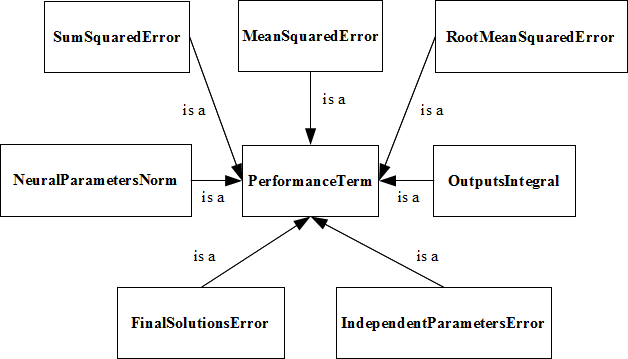
\includegraphics[width=1.1\textwidth]{performance_functional/performance_term_derived_diagram}
} \caption{Derived classes of the performance term.}\label{PerformanceTermDerivedClassDiagram}
\end{figure}

\subsection*{Attributes and operations}
\index{attribute, object oriented programming}
\index{operation, object oriented programming}

\subsubsection*{Data set}

A data-set has the following attributes:

\begin{itemize}
\item[-] A data matrix.
\item[-] A variables information object. 
\item[-] An instances information object.
\end{itemize}

It performs the following operations:

\begin{itemize}
\item[-] Load the data from a file.
\item[-] Scale/unscale the data.
\end{itemize}

\subsubsection*{Mathematical model}

A mathematical model has the following attributes:

\begin{itemize}
\item[-] The number of independent variables.
\item[-] The number of dependent variables.
\end{itemize}

It performs the following operations:

\begin{itemize}
\item[-] Calculate the solution of the mathematical model.
\end{itemize}

\subsubsection*{Performance term}

A performance term has the following attributes:

\begin{itemize}
\item[-] A relationship to a neural network. In C++ this is implemented as a pointer to a neural network object.
\item[-] An relationship to a data set.
\item[-] An relationship to a mathematical model.
\end{itemize}

It performs the following operations:

\begin{itemize}
\item[-] Calculate the evaluation of the performance term. 
\item[-] Calculate the derivatives of the performance term with respect to the neural network parameters.
\end{itemize}
   

\subsubsection*{Performance functional}

A performance functional for a neural network has the following attributes:

\begin{itemize}
\item[-] A relationship to a neural network. In C++ this is implemented as a pointer to a neural network object.
\item[-] An objective performance term.
\item[-] A regularization performance term.
\item[-] A constraints performance term.
\end{itemize}

It performs the following operations:

\begin{itemize}
\item[-] Calculate the performance of a neural network.
\item[-] Calculate the derivatives of the performance with respect to the parameters.
\end{itemize}


